% !TEX encoding = UTF-8 Unicode
% TEX TS-program = pdflatex
\documentclass{scrartcl}
\usepackage[utf8]{inputenc}

\usepackage{natbib}
\usepackage{url}
\usepackage{graphicx}

\usepackage{xcolor}
\definecolor{c9red}{RGB}{219,97,100}
\usepackage{tcolorbox}
\usepackage{etoolbox}
\usepackage{courier}

\usepackage{minted}
\BeforeBeginEnvironment{minted}{\begin{tcolorbox}}
\AfterEndEnvironment{minted}{\end{tcolorbox}}

\makeatletter
\DeclareOldFontCommand{\rm}{\normalfont\rmfamily}{\mathrm}
\DeclareOldFontCommand{\sf}{\normalfont\sffamily}{\mathsf}
\DeclareOldFontCommand{\tt}{\normalfont\ttfamily}{\mathtt}
\DeclareOldFontCommand{\bf}{\normalfont\bfseries}{\mathbf}
\DeclareOldFontCommand{\it}{\normalfont\itshape}{\mathit}
\DeclareOldFontCommand{\sl}{\normalfont\slshape}{\@nomath\sl}
\DeclareOldFontCommand{\sc}{\normalfont\scshape}{\@nomath\sc}
\makeatother

\usepackage{tikz}
\usetikzlibrary{shadows}

\newcommand*\keystroke[1]{%
  \tikz[baseline=(key.base)]
    \node[%
      draw,
      fill=white,
      drop shadow={shadow xshift=0.25ex,shadow yshift=-0.25ex,fill=black,opacity=0.75},
      rectangle,
      rounded corners=2pt,
      inner sep=1pt,
      line width=0.5pt,
      font=\scriptsize\sffamily
    ](key) {#1\strut}
  ;
}

\begin{document}

\title{Metagenomics ECCB 2018 Tutorial}
\subtitle{Part II: large scale sequence analysis}
\author{Clovis Galiez, Milot Mirdita, Martin Steinegger, Johannes Söding}
\date{Sept. 2018}

\maketitle

\section{Introduction}
MMseqs2 (Many-against-Many sequence searching \citep{steinegger2017mmseqs2}) is a software suite to search and cluster huge protein sequence sets. MMseqs2 is open source GPLv3-licensed software implemented in C\texttt{++} for Linux, macOS, and Windows. The software is designed to run on multiple cores and servers and exhibits very good scalability. MMseqs2 can run 10\,000 times faster than BLAST. At 50 times its speed it achieves almost the same sensitivity. It can perform profile searches with the same sensitivity as PSI-BLAST at over 400 times its speed.

\begin{figure}[h!]
\centering
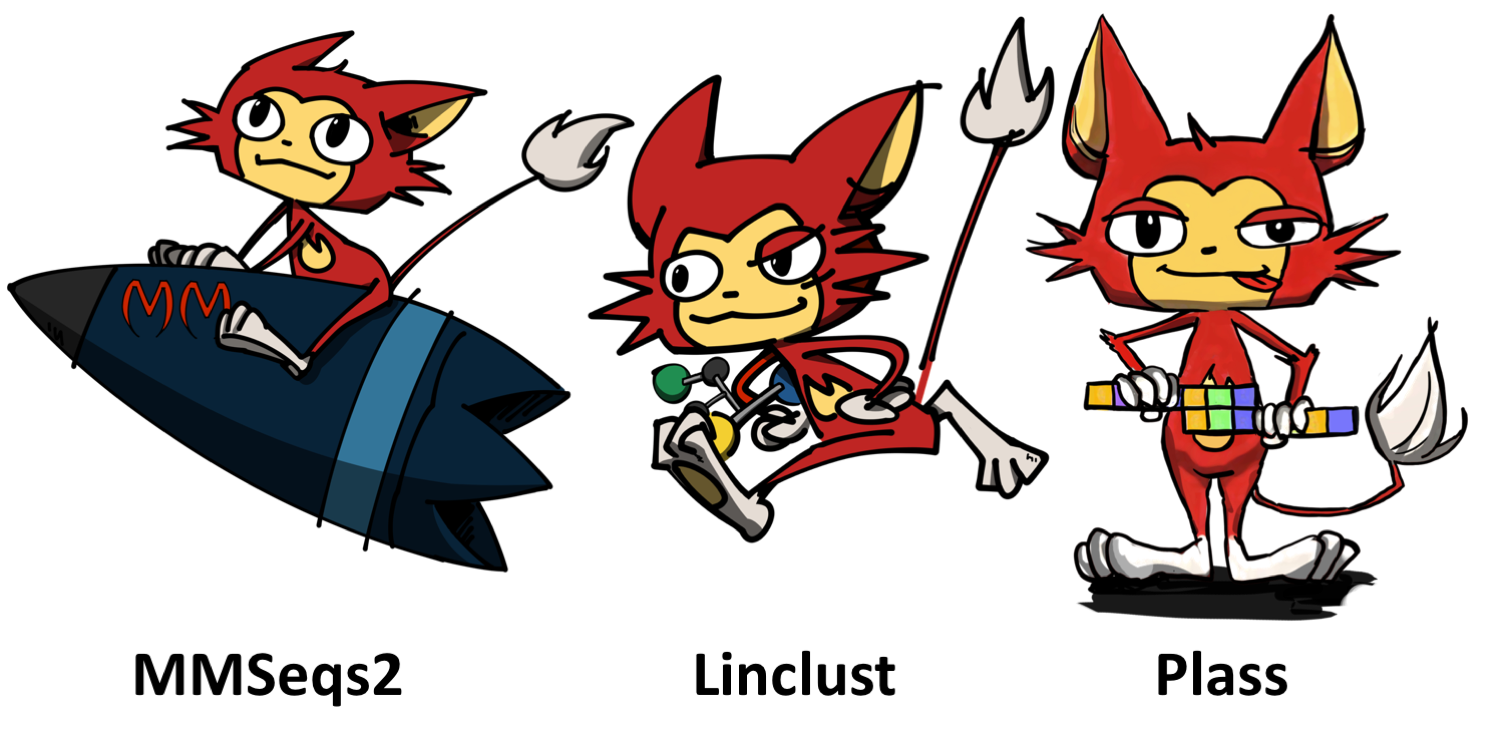
\includegraphics[height=70mm]{ThreeTools.png}
\caption{Your new friends! \textbf{MMseqs2} ultra fast and sensitive protein search, \textbf{Linclust} clustering huge protein sequence sets in linear time and \textbf{Plass} Protein-level assembly to increases protein sequence recovery from complex metagenomes}
\label{fig:universe}
\end{figure}

Here you will learn the basic usage of MMseqs2 as well as expert tricks to take advantage of the ability of chaining different MMseqs2 modules to produce custom workflows. We will show on a human gut metagenomic dataset (SRA run \texttt{ERR1384114}) what the advantages of using Linclust (linear time clustering algorithm, \cite{Steinegger:2018aa}), Plass (Protein Level Assembly,  \cite{Steinegger386110}) and MMseqs2 are over the more conventional pipeline with MegaHit\citep{li2015megahit}, Prodigal\citep{hyatt2010prodigal} and HMMER\citep{eddy2009new}.

\section{Discover your environment}
\subsection{Command line interface and software}
You will work on your own remote virtual machine through a Bash terminal in your browser. You will use the same environment as in the morning session. Please navigate to the \textbf{\texttt{\$HOME/mmseqs2tutorial}} directory. All software and data has already been set up there. The commands to reproduce the installation are available in the file \texttt{scripts/setup.sh} on GitHub of the tutorial \url{https://github.com/soedinglab/metaG-ECCB18-partII}.

The software is installed in the \texttt{software} subdirectory and integrated in your \texttt{\$PATH} environment variable.

You can take a look at the following commands:
\begin{minted}{bash}
plass
mmseqs
megahit -h
prodigal
\end{minted}

The generic syntax for \texttt{mmseqs} and \texttt{plass} calls is always the following:
\begin{minted}{bash}
mmseqs <command> <db1> [<db2> ...] --flag --parameter 42
\end{minted}

The help text of \texttt{mmseqs} shows, by default, only the most important parameters and modules. To see a full list of parameters and modules use the \texttt{-h} flag. You can auto complete commands and parameters of \texttt{mmseqs} by using the \keystroke{tab} key. 

The FASTQ read file you are going to work on is in the \texttt{data} directory.

\section{Analysis of a human gut metagenomics dataset}
\subsection{Getting a protein catalogue of a metagenome}
We use Plass to assemble a catalogue of protein sequences directly from the reads, without the nucleic assembly step. It recovers 2 to 10 times more protein sequences from complex metagenomes than other state-of-the-art methods and can assemble huge datasets. 

The standard genomic assemblies prevent many reads to assemble due to  \textbf{low coverages} and \textbf{micro-diversity}. To run this protein-level assembly, use the command

\begin{minted}{bash}
plass assemble data/ERR1384114.fastq plassProteins.faa tmpDir
\end{minted}

or type \texttt{plass assemble -h} to see all available options.

\vspace{1em}
As a matter of comparison, run the usual pipeline using MegaHit for genomic assembly:

\begin{minted}{bash}
megahit -r ERR1384114.fastq -o megahitAssemblyOutput
\end{minted}

Then extract the proteins using Prodigal:
\begin{minted}{bash}
prodigal -i megahitAssemblyOutput/final.contigs.fa\
    -a prodigal.faa -p meta
\end{minted}

Take a look at the FASTA files produced by Plass and Prodigal. To check the number of detected proteins, you can count the number of FASTA headers (lines beginning with the \texttt{\textgreater} character):

\begin{minted}{bash}
grep -c "^>" file.faa
\end{minted}

\paragraph{Redundancy reduction}
Since Plass assembles with replacement of reads, the catalogue will contain some redundancy. You can reduce this catalogue by clustering it, for instance, to 90\% of sequence identity, and asking for the representative sequence that cover at least 95\% of the members. For this, you can either use the \texttt{easy-cluster} (sensitive clustering) or \texttt{easy-linclust} (linear time fast clustering) modules of MMseqs2:
\begin{minted}{bash}
mmseqs easy-cluster plassProteins.faa clusteredProts.faa \
    tmpDir --min-seq-id 0.9 -c 0.95 --cov-mode 1
\end{minted}

Both the default MMseqs2 clustering and Linclust link two sequences by an edge based on three local alignment criteria:
\begin{itemize}
\item a maximum E-value threshold (option \texttt{-e}, default $10^{-3}$) computed according to the gap-corrected Karlin-Altschul statistics;

\item a minimum coverage (option \texttt{-c}, which is defined by the number of aligned residue pairs divided by either the maximum of the length of query/centre and target/non-centre sequences alnRes/max(qLen,tLen) (default mode, \texttt{-{}-cov-mode} 0), by the length of the target/non-centre sequence alnRes/tLen (\texttt{-{}-cov-mode} 1), or by the length of the query/centre alnRes/qLen (\texttt{-{}-cov-mode 2});

\item a minimum sequence identity (\texttt{-{}-min-seq-id}) with option \texttt{-{}-alignment-mode} defined as the number of identical aligned residues divided by the number of aligned columns including internal gap columns, or, by default, defined by a highly correlated measure, the equivalent similarity score of the local alignment (including gap penalties) divided by the maximum of the lengths of the two locally aligned sequence segments. The score per residue equivalent to a certain sequence identity is obtained by a linear regression using thousands of local alignments as training set.
\end{itemize}

You can count the number of entries in your clustered FASTA file \\ \texttt{clusteredProts.faa\_all\_seqs.faa} again using the previous \texttt{grep} command.

\paragraph{Learn how to deal with MMseqs2's indexed databases} The previous \texttt{easy-cluster} command is a shorthand to deal directly with FASTA files as input and output. However, MMseqs2's modules \textbf{do not} use the FASTA format internally. Since the goal of this tutorial is to make you an expert in using MMseqs2 workflows, we will explain and use the MMseqs2 database formats and create FASTA files only for downstream tools.

You can convert a FASTA file to the MMseqs2 database format using:
\begin{minted}{bash}
mmseqs createdb plassProteins.faa plassProteinsDb
\end{minted}

This generates several files: a \textit{data} file \texttt{plassProteinsDb} together with an \textit{index} file \texttt{plassProteinsDb.index}. The first file contains all the sequences separated by a null byte \texttt{\textbackslash0}. We coin more generally any data record \textit{an entry}, and each entry is associated with a unique \textit{key} (integer number) that is stored in the \textit{index} file.

\begin{figure}[h!]
\centering
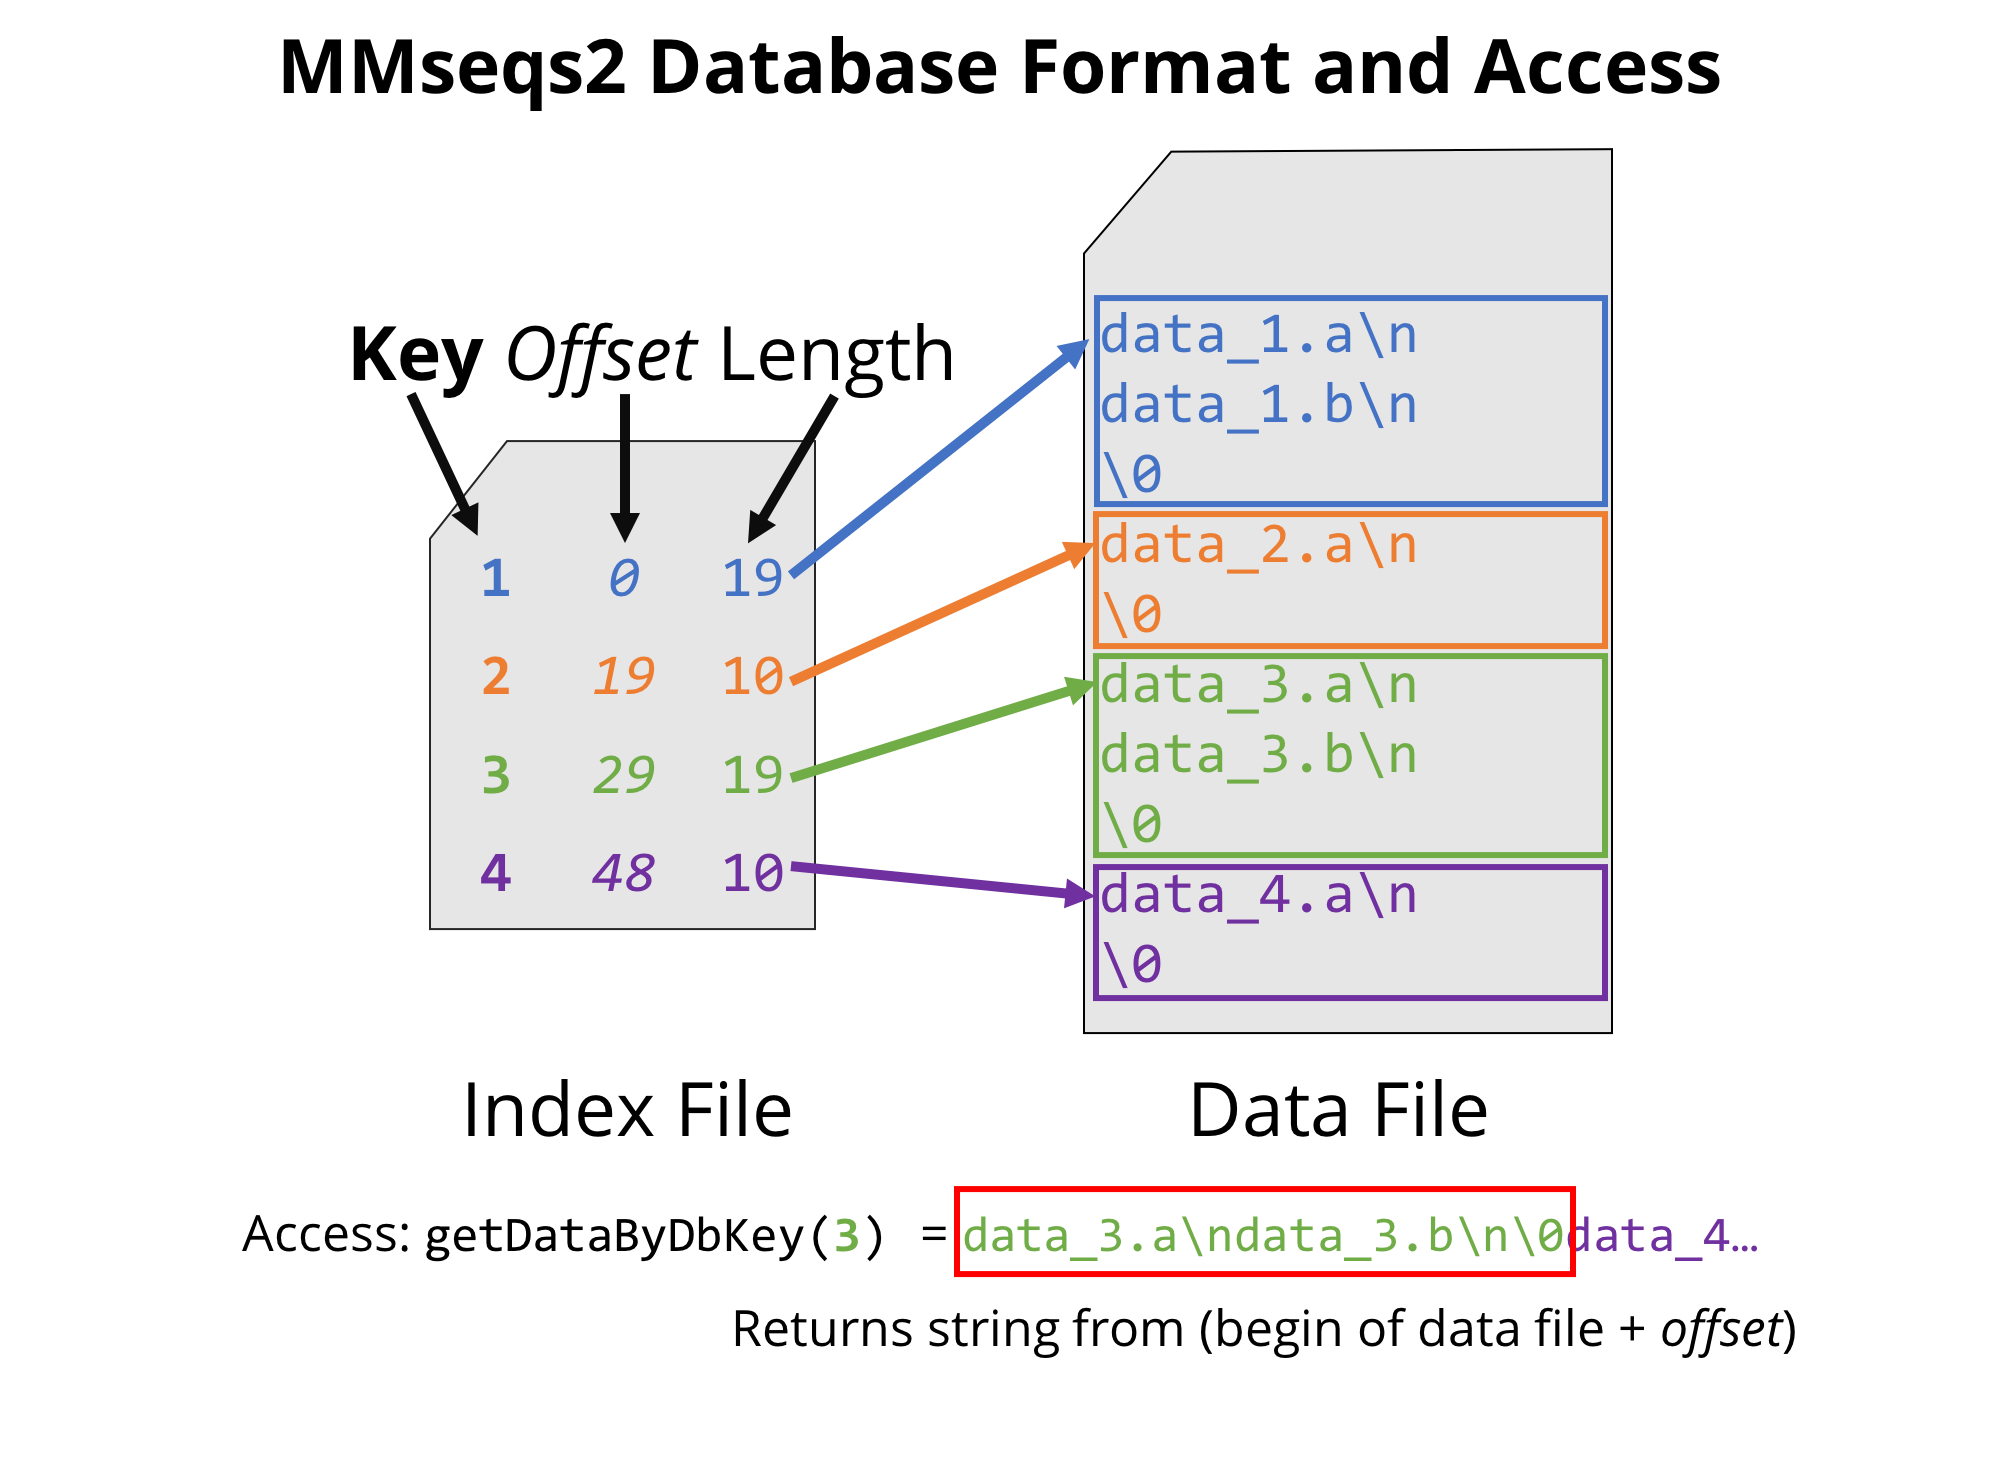
\includegraphics[height=70mm]{mmseqs-db-format}
\caption{MMseqs2 database format, through which all MMseqs2 modules can be easily and efficiently chained.}
\label{fig:dbformat}
\end{figure}

The corresponding headers are stored in a separate database with a \texttt{\_h} suffix (\texttt{plassProteinsDb\_h}).

The \texttt{.dbtype} file helps to keep track of the database type (amino-acid, nucleic, profile, etc.).

The \texttt{.lookup} file is a lookup file linking the keys to their sequence accession as specified in their FASTA header.

The format of this index file is tab-separated and reports one line per entry in the database, specifying a unique key (column 1), the offset and the length of the corresponding data (columns 2 and 3 respectively). As we will make use of the efficient structure later on in the tutorial, you can already take a look at the index file structure with:

\begin{minted}{bash}
head plassProteinsDb.index
\end{minted}

We provide a simple bash function to access a single entry of the file.

With it, you can access data for \textit{an entry} with the \texttt{getentry} command. This command takes the data filename (e.g. plassProteinsDb) and the \texttt{ENTRYOFFSET} (second column of the index) and the \texttt{ENTRYLENGTH} (third column of the index). Please try to access a single entry of the datafile. 

\begin{minted}{bash}
getentry FILENAME ENTRYOFFSET ENTRYLENGTH 
\end{minted}


Let's re-run the clustering of the catalogue database with our fresh database:
\begin{minted}{bash}
mmseqs cluster plassProteinsDb plassProteinsReduced tmpDir \
    --min-seq-id 0.9 -c 0.95 --cov-mode 1 
\end{minted}

This creates a \textit{cluster database} where \textbf{each entry has the key of its representative sequence}, and whose data consists of the list of keys of its members:
\begin{minted}[texcomments]{bash}
# the index file contains entries whose
# keys are of those of their representative sequence
head plassProteinsReduced.index 

# you will see the keys belonging to different clusters
# (one per line) and such that every cluster is
# separated by a null byte (shown as a \colorbox{c9red}{\color{white}{\textbullet}} in your C9 IDE
# or as \textasciicircum@ in vim
c9 open plassProteinsReduced
\end{minted}

\textit{Note:} This is a general principle in MMseqs2: the keys are always consistent between databases (input and output, clustering and sequence databases, and potentially intermediate files.

Therefore, to count the number of clusters, you can count the number of lines in the \textit{index} file using:
\begin{minted}{bash}
wc -l plassProteinsReduced.index
\end{minted}

\subsection{Annotating the catalogue}
To get domain annotation for your protein catalogue, we search the sequences against a database of Pfam profiles:
\begin{minted}{bash}
# first create a sequence database of
# the representative sequences
cat plassProteinsReduced.index > keysOfRepSeq
#  sequence db
mmseqs createsubdb keysOfRepSeq plassProteinsDb\
    plassProteinsNr
#  do the same for its headers
mmseqs createsubdb keysOfRepSeq plassProteinsDb_h \
    plassProteinsNr_h


# -s 7 for high sensitivity
mmseqs search plassProteinsNr \
    $HOME/mmseqs2tutorial/databases/pfamProfiles \
    searchOutProfile.mmseqs tmp -s 7 --no-preload

# you can make it human-readable in TSV format
mmseqs createtsv plassProteinsNr \
    $HOME/mmseqs2tutorial/databases/pfamProfiles \
    searchOutProfile.mmseqs searchOutProfile.mmseqs.tsv
\end{minted}


\paragraph{Learn how to filter databases}
You can post-process the annotation file to retrieve only annotations of high confidence:
\begin{minted}{bash}
# check that the e-values are shown in column 4
# of the search result file
head searchOutProfile.mmseqs

# create a new database containing
# only annotations of e-value <= 1e-5
mmseqs filterdb searchOutProfile.mmseqs \
    strongPfamAnnotations --filter-column 4 \
    --comparison-operator le --comparison-value 1e-5
\end{minted}

An advanced way to extract the entries that did not get a reliable annotation uses the fact that if no hit was found for a given sequence, the corresponding entry in the \textit{data file} will be empty, resulting in a data length of 1 (for the null byte) in the \textit{index file}:
\begin{minted}{bash}
# extract the keys of entries having
# no annotation better than 1e-5
awk '$3==1 {print $1}' strongPfamAnnotations.index \
   > uncertainFunction.keys

# create a FASTA file for further investigation
# in downstream tools (HHblits for instance)

# First extract sub-database containing
# the protein sequences of uncertain function
#   - sequence db
mmseqs createsubdb uncertainFunction.keys plassProteinsNr \
    plassProteinsNr.uncertainFunc
#   - do the same for its headers
mmseqs createsubdb uncertainFunction.keys plassProteinsNr_h \
    plassProteinsNr.uncertainFunc_h

# convert it to a fasta file
mmseqs convert2fasta plassProteinsNr.uncertainFunc \
    plassProteinsNr.uncertainFunc.faa
\end{minted}

\paragraph{What is the difference to standard annotation tools?}

You can compare (time and number of annotation) with HMMER3:
\begin{minted}{bash}
time hmmscan --notextw --noali --tblout "hmmer.tblout" \
    --domtblout "hmmer.domtblout" \
    $HOME/mmseqs2tutorial/databases/Pfam-A.full_hmmer \
    clusteredProts.faa 

# check the number of annotated proteins
#   for MMseqs2
awk '$3 > 1 {print $1}' searchOutProfile.mmseqs.index|wc -l
#   for HMMER
tail -n+4 hmmer.tblout | cut -c 21-30 | sort -u | wc -l 
\end{minted}


\section{Build you own workflows}
\subsection{Cascaded profile clustering (deep clustering)}
We will take advantage of MMseqs2's \textbf{modular architecture} to create a workflow (bash script) that calls MMseqs2 tools to deeply cluster a set of proteins. 

\paragraph{Cascaded sequence clustering} Let's first create a cascaded clustering workflow: after a first clustering step, the representative sequences of each of the clusters are searched against each other and the result of the search is again clustered. By repeating this procedure iteratively, one gets a deeper clustering of the original set.

Try to code complete the following script:
\begin{minted}{bash}
#!/bin/bash -e

inputdb="plassProteinsReduced"
for step in {1..maxStep}; do
    # we do not use the cluster mmseqs command as it
    # already is a cascaded workfolw clustering
    mmseqs search $inputdb $inputdb searchStep$step tmpDir
    mmseqs clust $inputdb searchStep$step clusteringStep$step
    mmseqs result2repseq ...
    inputdb=...
done

# Then merge the clustering steps
mmseqs mergeclusters plassProteinsReduced deepClusterDB ...
\end{minted}

Try your script with 3 steps, and check the clustering depth (number of clusters) at each step:
\begin{minted}{bash}
wc -l clusteringStep*.index
\end{minted}

What do you notice ?

\paragraph{Deeper clustering using profiles}
To make a deeper clustering of your protein set, one idea is to create a cascaded clustering where the sequence search at every iteration is replaced by a profile to sequence search (more sensitive search than sequence to sequence searches). Write your own workflow that will be using the \texttt{result2profile} module. After adjusting your workflow to handle profiles also add the \texttt{--add-self-matches} parameter to the search to assure that the query is contained in each search results.

Did you manage to cluster more deeply?

You can get the distribution of your cluster sizes by calling:

\begin{minted}{bash}
# get the size of every cluster
mmseqs result2stats plassProteinsReduced plassProteinsReduced \
    deepClusterDB deepClusterDB.clusterSizes --stat linecount
# show the distribution
tr -d '\0' < deepClusterDB.clusterSizes | sort -n | uniq -c
\end{minted}

Compare this clustering to your first cascaded clustering.

\subsection{Abundance analysis}
Let's check the most abundant genes in our dataset. To this end, we want to map the ORFs from the reads to the protein catalogue, and count the number of hits on each of the proteins.

Write an MMseqs2 workflow that:
\begin{itemize}
    \item creates a read sequence database from the FASTA files (\texttt{createdb})
    \item extracts the ORFs from the read database (\texttt{extractorfs}),
    \item translate the nucleotide ORFs to protein sequences (\texttt{translatenucs}),
    \item map them on the proteins (\texttt{prefilter} with option \texttt{-s 2} since mapping calls for high sequence identity),
    \item score the prefilter hits with a gapless alignment (\texttt{rescorediagonal} with option \texttt{-c 1 --cov-mode 2 --min-seq-id 0.95 --rescore-mode 2 -e 0.000001 --sort-results 1} to have significant hits and fully covered by the protein sequence),
    \item keep the best mapping target (\texttt{filterdb} with flag \texttt{--extract-lines 1}),
    \item in the database output from the last step, every entry is a read-ORF. Now you should transpose the database so that each contig is an entry, and the data is the list of mapped read-ORFs (\texttt{swapresults}),
    \item count the number of mapped read-ORF (\texttt{result2stats}). Advanced: instead of just count the reads, sum up the aligned length and divide it by the contig length \texttt{apply} and \texttt{awk}. The contig length and alignment length (alnEnd - alnStart) is in the alignment format.
\end{itemize}

We can use \texttt{createtsv} to output the abundances as a TSV formatted file:
\begin{minted}{bash}
# Create a flat file
mmseqs createtsv plassProteinsReduced plassProteinsReduced\
    mapAbundances mapAbundances.tsv --target-column 0
\end{minted}

\subsection{Re-create the linclust workflow... if you have time :)}

Based on the explanation of the Linclust algorithm, try to code its workflow using:
\begin{itemize}
    \item \texttt{kmermatcher}
    \item \texttt{rescorediagonal}
    \item \texttt{clust}
\end{itemize}

Take a look at the real Linclust workflow in \url{\$HOME/mmseqs2tutorial/software/MMseqs2/data/linclust.sh}. This version is slightly more involved as it integrates a redundancy reduction step (the \texttt{pre\_clust} prefiltering by high Hamming distance), and uses a trick using \texttt{filterdb} with the flag  \texttt{--filter-file} to apply the workflow you just built \textit{only} on the \textit{non-redundant} entries. At the end of the file, you can also spot a merging step to recover the redundant part in the final clustering.

\section{Conclusion}
We hope that you are more familiar with the MMseqs2 environment, and that you enjoy its modularity and flexibility for creating new workflows. Due to time and virtual machine constraints we chose a rather small metagenomic dataset, but using MMseqs2 on bigger datasets should convince you of its scalability.

Please help us by giving critical feedback on this tutorial!

\bibliographystyle{natbib}
\bibliography{references}
\end{document}
